\documentclass{standalone}

\usepackage{tikz}
\usetikzlibrary{arrows.meta,
                calc, chains,
                quotes,
                positioning,
                shapes.geometric}

\begin{document}

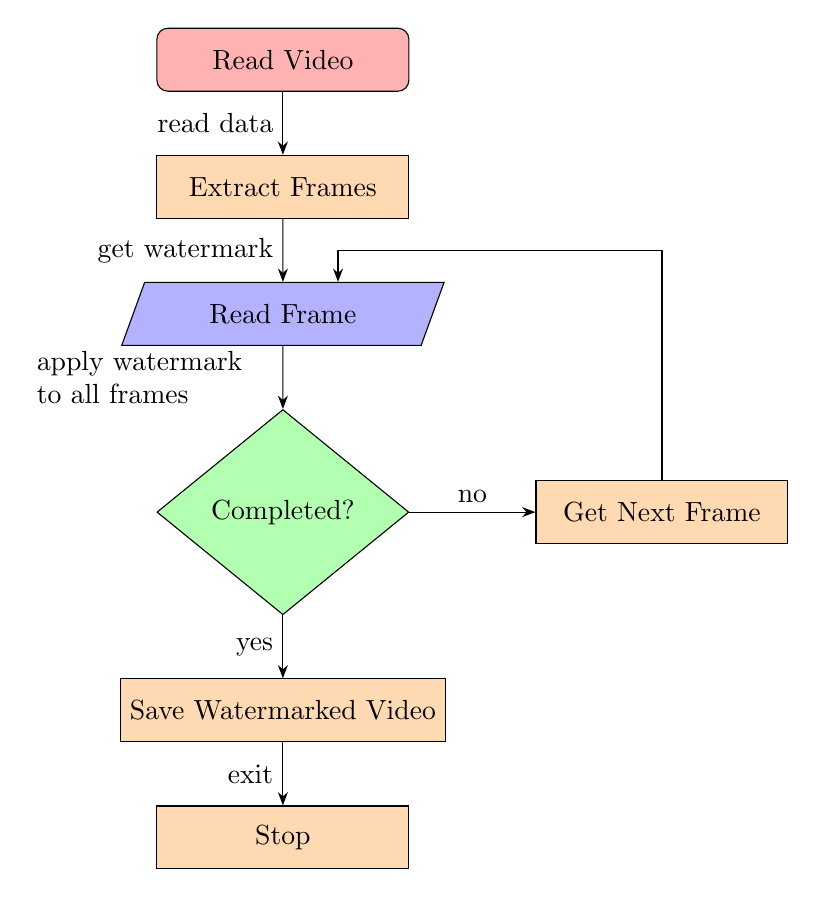
\begin{tikzpicture}[
    node distance = 8mm and 16mm,
      start chain = A going below,
      base/.style = {draw, minimum width=32mm, minimum height=8mm,
                     align=center, on chain=A},
 startstop/.style = {base, rectangle, rounded corners, fill=red!30},
   process/.style = {base, rectangle, fill=orange!30},
        io/.style = {base, trapezium, 
                     trapezium left angle=70, trapezium right angle=110,
                     fill=blue!30},
  decision/.style = {base, diamond, fill=green!30},
  every edge quotes/.style = {auto=right}]
                    ]
\node [startstop]       {Read Video};            % <-- A-1
\node [process]         {Extract Frames};
\node [io]              {Read Frame};
\node [decision]        {Completed?};
\node [process]         {Save Watermarked Video};
\node [process]         {Stop};             % <-- A-6
%
\node [process,                             % <-- A-7
       right=of A-4]    {Get Next Frame};
%%
\draw [arrows=-Stealth] 
    (A-1) edge["read data"]          (A-2)
    (A-2) edge["get watermark"]    (A-3)
    (A-3) edge[text width=3cm,"apply watermark to all frames "]       (A-4)
    (A-4) edge["yes"]            (A-5)
    (A-5) edge["exit"]          (A-6)
    (A-4) edge["no"']          (A-7)       % <-- by ' is swapped label position
    (A-7) |- ($(A-2.south east)!0.5!(A-3.north east)$)
          -| ([xshift=7mm] A-3.north)
    ;
  \end{tikzpicture}
\end{document}